\documentclass[11pt,twocolumn]{article}
\usepackage[margin=0.75in]{geometry}
\usepackage{cite}
\usepackage{amsmath,amssymb,amsfonts}
\usepackage{algorithmic}
\usepackage{graphicx}
\usepackage{textcomp}
\usepackage{xcolor}
\usepackage{hyperref}
\usepackage{booktabs}
\usepackage{multirow}
\usepackage{array}
\usepackage{authblk}

\def\BibTeX{{\rm B\kern-.05em{\sc i\kern-.025em b}\kern-.08em
    T\kern-.1667em\lower.7ex\hbox{E}\kern-.125emX}}

\begin{document}


\title{TrendScout AI: A Hybrid RAG and Knowledge Graph System for Conversational Market Intelligence in AI Startups}

\author[1]{Aditya Pokharna}
\author[1]{Sahil Pawar}
\author[1]{Wei-An Wang}
\author[1]{Yu-Yao Hsieh}
\author[1]{Zih-Jyun Lin}
\affil[1]{School of Computing and Augmented Intelligence, Arizona State University, Tempe, Arizona, USA}

\date{November 26, 2025}

\maketitle

\begin{abstract}
The artificial intelligence startup ecosystem has experienced unprecedented growth, with AI companies raising \$56 billion in 2024 alone, representing 46.4\% of total US venture capital funding. This explosive growth has created significant information overload for investors, analysts, and industry stakeholders who struggle to track funding rounds, product launches, partnerships, and rapidly evolving industry narratives. We present TrendScout AI, a conversational market intelligence system that combines Retrieval-Augmented Generation (RAG) with Knowledge Graph (KG) technologies to provide intelligent, context-aware responses about AI startups. Our hybrid approach leverages ChromaDB for semantic vector search and Neo4j for structured relationship queries, synthesizing information through GPT-4 to deliver comprehensive answers. Through systematic evaluation on 50 diverse questions across five categories (factual, relationship, comparison, temporal, and detail queries), we demonstrate that our RAG+KG hybrid system significantly outperforms RAG-only approaches, achieving a 44\% win rate compared to 14\% for RAG-only, with an average improvement of 1.64 points on a 15-point scale. The system shows particularly strong performance on factual queries (+2.8 points) and relationship queries (+3.3 points), demonstrating the value of structured knowledge representation for market intelligence applications.
\end{abstract}

\noindent\textbf{Keywords:} Retrieval-Augmented Generation, Knowledge Graph, Natural Language Processing, Market Intelligence, Conversational AI, Neo4j, Vector Databases

\section{Introduction}

The artificial intelligence industry has entered a transformative phase characterized by rapid innovation, massive capital influx, and intense competition. In 2024, generative AI startups alone raised \$56 billion, reflecting growing investor confidence in AI technologies \cite{pitchbook2024}. This unprecedented growth has fundamentally altered the venture capital landscape, with 46.4\% of US VC funding now directed toward AI companies, up from 36\% in previous years \cite{cbinsights2024}. Venture capitalists themselves have embraced AI tools, with 76\% using AI for daily operations and 62\% leveraging AI to research potential investment opportunities \cite{vcsurvey2024}.

However, this explosive growth has created substantial challenges for market participants. The sheer volume of information—funding announcements, product launches, strategic partnerships, technical breakthroughs, and evolving industry narratives—has overwhelmed traditional manual tracking methods. Industry trends shift rapidly; themes like "AI agents" and "AI infrastructure" emerge and evolve within months, making it difficult for investors and analysts to maintain current, comprehensive understanding of the competitive landscape.

Traditional approaches to market intelligence rely heavily on manual research, requiring analysts to aggregate information from disparate sources including news articles, company announcements, LinkedIn posts, and industry reports. This process is time-consuming, prone to information gaps, and struggles to capture the complex relationships between companies, products, partnerships, and technologies that characterize the modern AI ecosystem.

Recent advances in Large Language Models (LLMs) and semantic search technologies have opened new possibilities for automated market intelligence. Retrieval-Augmented Generation (RAG) systems can retrieve relevant context from document collections and generate informed responses, while Knowledge Graphs excel at representing and querying structured relationships between entities. However, each approach has inherent limitations when applied in isolation to complex market intelligence tasks.

We present TrendScout AI, a novel hybrid system that synergistically combines RAG and Knowledge Graph technologies to address these challenges. Our system analyzes LinkedIn posts from leading AI companies—Perplexity AI, OpenAI, Anthropic, Mistral AI, and DeepSeek—to build both a vector database for semantic search and a structured knowledge graph for relationship queries. By intelligently routing queries to appropriate retrieval mechanisms and synthesizing results through GPT-4, TrendScout AI provides accurate, comprehensive, and contextually relevant answers to natural language questions about the AI startup ecosystem.

The key contributions of this work are:

\begin{itemize}
\item A hybrid RAG+KG architecture specifically designed for market intelligence applications, combining semantic search capabilities with structured relationship queries
\item An LLM-powered entity extraction pipeline using Google's Gemini API that automatically constructs knowledge graphs from unstructured social media content
\item A comprehensive evaluation framework with 50 carefully designed questions across five distinct categories, enabling systematic comparison of different retrieval approaches
\item Empirical evidence demonstrating significant performance improvements of hybrid RAG+KG systems over RAG-only approaches, particularly for factual and relationship-based queries
\item A production-ready web interface with configurable retrieval options, enabling users to compare different system configurations in real-time
\end{itemize}

The remainder of this paper is organized as follows: Section II presents the problem statement in detail, Section III reviews related work in RAG systems and knowledge graphs, Section IV describes our system architecture and algorithms, Section V details our datasets and preprocessing methods, Section VI presents comprehensive evaluation results, Section VII showcases our user interface design, Section VIII describes team member contributions, and Section IX concludes with future directions.

\section{Problem Statement}

The rapid evolution of the AI startup ecosystem presents several interconnected challenges that existing market intelligence solutions inadequately address:

\textbf{Information Overload and Fragmentation:} Market participants face an overwhelming volume of information distributed across multiple platforms and formats. AI companies announce developments through LinkedIn posts, Twitter threads, blog posts, press releases, and conference presentations. Investors and analysts must manually aggregate this fragmented information, a process that is both time-consuming and prone to missing critical updates.

\textbf{Complex Relational Queries:} Understanding the AI startup landscape requires answering complex relational questions such as "Which companies have partnerships with government agencies?" or "What are the competitive dynamics between Perplexity AI and OpenAI in the search market?" These queries require not just finding relevant documents, but understanding and reasoning about relationships between entities—companies, products, partnerships, and technologies.

\textbf{Temporal Dynamics:} Industry narratives and competitive positioning evolve rapidly. A comprehensive market intelligence system must track temporal patterns, identify emerging trends, and provide current information while maintaining historical context. Static databases or infrequently updated reports fail to capture this dynamic nature.

\textbf{Contextual Understanding:} Effective market intelligence requires deep contextual understanding. When an AI company announces a new product feature, analysts need to understand how it relates to the company's existing product portfolio, how it compares to competitor offerings, and what strategic implications it carries for the market.

\textbf{Limitations of Existing Approaches:} Traditional manual research methods cannot scale to the volume and velocity of information in the modern AI ecosystem. Pure keyword search lacks semantic understanding and struggles with synonyms and varied terminology. RAG-only systems, while powerful for semantic search, do not explicitly capture or leverage structured relationships between entities. Knowledge Graph-only approaches require extensive manual curation and may miss nuanced contextual information present in natural language descriptions.

Our work addresses these challenges by developing a hybrid system that combines the semantic understanding capabilities of RAG with the structured relationship representation of Knowledge Graphs. We specifically focus on answering the research question: \textit{Can a hybrid RAG+KG approach significantly improve the accuracy and completeness of responses to diverse market intelligence queries compared to RAG-only systems, and for which types of queries is each approach most effective?}

\section{Related Works}

\subsection{Retrieval-Augmented Generation}

Retrieval-Augmented Generation (RAG) has emerged as a powerful paradigm for enhancing Large Language Models with external knowledge. Lewis et al. \cite{lewis2020rag} introduced the foundational RAG architecture, combining neural retrieval with sequence-to-sequence models to ground generation in retrieved documents. This approach addresses the key limitation of pure LLMs—their reliance on parametric knowledge frozen at training time—by dynamically retrieving relevant context at inference time.

Recent advances in RAG systems have focused on improving retrieval quality and generation fidelity. Gao et al. \cite{gao2023rag} demonstrated that dense retrieval using learned embeddings substantially outperforms traditional sparse methods like BM25 for complex queries. Shi et al. \cite{shi2023replicable} showed that chunk size and overlap strategies significantly impact retrieval effectiveness, with smaller chunks (256-512 tokens) generally performing better for precise fact retrieval.

Several studies have explored domain-specific RAG applications. Xiong et al. \cite{xiong2023medrag} developed MedRAG for medical question answering, demonstrating the importance of domain-adapted retrieval indices. In the financial domain, Wu et al. \cite{wu2023finrag} showed that RAG systems can effectively synthesize information from financial reports and market data, though they noted challenges with temporal queries and relationship extraction.

\subsection{Knowledge Graphs for Information Retrieval}

Knowledge Graphs provide structured representations of entities and relationships, enabling sophisticated reasoning and query capabilities. Neo4j and other graph databases have been widely adopted for applications requiring complex relationship queries \cite{robinson2015graph}. In the context of market intelligence, several systems have demonstrated the value of knowledge graph representations.

Färber et al. \cite{farber2018linkedeconomy} developed LinkedEconomy, a knowledge graph of economic entities and relationships, demonstrating how structured representations enable complex analytical queries. Ristoski et al. \cite{ristoski2016rdf2vec} introduced RDF2Vec, combining knowledge graph structure with embedding techniques to support similarity search and entity classification.

However, pure knowledge graph approaches face significant challenges. Manual curation is expensive and cannot scale to rapidly evolving domains. Automated knowledge graph construction from text remains challenging, with entity extraction and relationship identification requiring sophisticated NLP techniques \cite{rosso2022entity}.

\subsection{Hybrid Approaches}

Recent work has begun exploring hybrid systems that combine retrieval-based and structured knowledge approaches. Baek et al. \cite{baek2023knowledge} proposed Knowledge-Augmented Language Models that jointly leverage parametric knowledge, retrieved text, and knowledge graph triples, showing improvements on knowledge-intensive tasks.

Sun et al. \cite{sun2023text} introduced a framework for enhancing text-to-SQL generation with knowledge graphs, demonstrating that structured knowledge can guide the interpretation of natural language queries. Similarly, Yasunaga et al. \cite{yasunaga2022linkbert} developed methods for pre-training language models with knowledge graph structure, improving performance on relationship-focused tasks.

Most directly relevant to our work, Pan et al. \cite{pan2023unifying} explored unifying retrieval and reasoning over text and knowledge graphs for open-domain question answering. They showed that different query types benefit from different retrieval mechanisms, with factual queries favoring knowledge graph retrieval and contextual queries benefiting from text retrieval.

Our work extends these hybrid approaches specifically for market intelligence applications, introducing an LLM-powered entity extraction pipeline for automated knowledge graph construction from social media content, and providing comprehensive evaluation across diverse query types to characterize when each retrieval mechanism provides maximum value.

\section{System Architecture and Algorithms}

Our system architecture implements a sophisticated hybrid retrieval pipeline that intelligently combines RAG and Knowledge Graph capabilities. Figure \ref{fig:dataflow} illustrates the complete data flow from collection through answer generation.

\begin{figure*}[t]
\centering
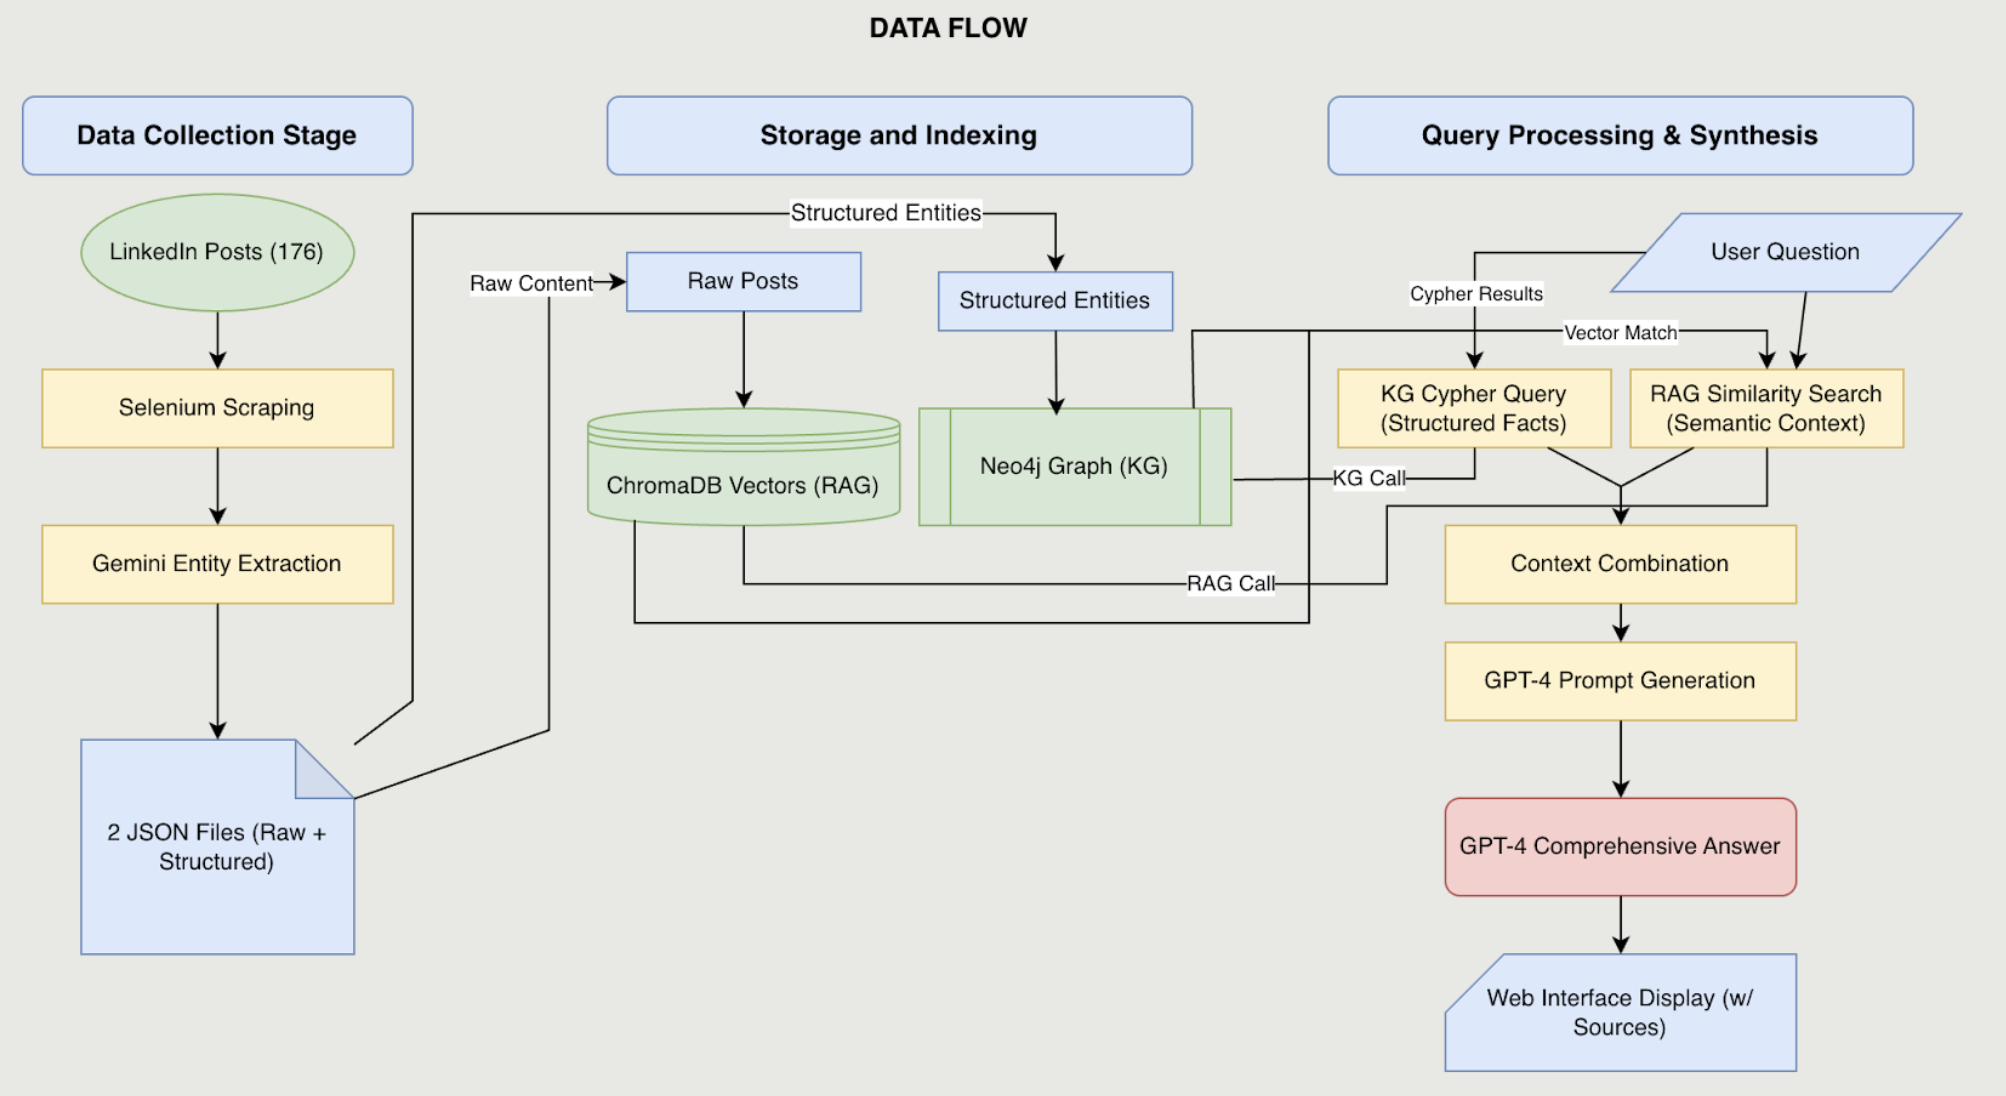
\includegraphics[width=\textwidth]{DataFlow.png}
\caption{Complete Data Flow Architecture: From LinkedIn post collection through Selenium scraping and Gemini entity extraction, to dual storage in ChromaDB and Neo4j, culminating in GPT-4 answer synthesis. The system processes user queries through both RAG similarity search and KG Cypher queries before combining contexts for comprehensive responses.}
\label{fig:dataflow}
\end{figure*}

\subsection{Overall Architecture}

The TrendScout AI system consists of five main components:

\begin{enumerate}
\item \textbf{Data Collection Layer:} Web scraping infrastructure for gathering LinkedIn posts
\item \textbf{Entity Extraction Layer:} LLM-powered processing to extract structured entities and relationships
\item \textbf{Dual Storage Layer:} Parallel storage in ChromaDB (vector database) and Neo4j (graph database)
\item \textbf{Intelligent Query Router:} Context-aware routing and retrieval from appropriate storage systems
\item \textbf{Answer Synthesis Layer:} GPT-4-based generation combining results from both retrieval mechanisms
\end{enumerate}

\subsection{Data Collection Pipeline}

We implemented a robust web scraping system using Selenium WebDriver and BeautifulSoup to collect LinkedIn company posts. The scraping process handles dynamic content loading, authentication, and rate limiting to ensure reliable data collection while respecting platform constraints.

\begin{verbatim}
Algorithm 1: LinkedIn Post Scraping
Input: company_urls, max_posts_per_company
Output: raw_posts

for each company in company_urls:
    driver = initialize_selenium()
    navigate_to(company.linkedin_page)
    scroll_and_load_posts(max_posts)
    posts = []
    for post in visible_posts:
        extract_text(post)
        extract_timestamp(post)
        extract_engagement_metrics(post)
        posts.append(post_data)
    raw_posts[company] = posts
return raw_posts
\end{verbatim}

\subsection{LLM-Powered Entity Extraction}

A critical innovation in our system is the use of Google's Gemini API for entity extraction. Traditional named entity recognition approaches struggle with the informal, varied language of social media posts. LLM-based extraction provides superior accuracy by understanding context and inferring implicit relationships.

Our extraction pipeline processes each post through a carefully designed prompt that instructs the LLM to identify:

\begin{itemize}
\item \textbf{Companies:} Primary company and any mentioned partners or competitors
\item \textbf{Products:} Product names, features, and capabilities
\item \textbf{AI Models:} Specific model names and versions
\item \textbf{Partners:} Organizations mentioned in partnership contexts
\item \textbf{Features:} Specific capabilities or technical features
\item \textbf{Topics:} High-level themes and categories
\end{itemize}

The LLM returns structured JSON output that is validated and normalized before storage. This approach achieves significantly higher accuracy than rule-based or traditional NER methods, particularly for handling acronyms, informal names, and implicit references.

\begin{verbatim}
Algorithm 2: LLM Entity Extraction
Input: post_text
Output: structured_entities

prompt = construct_extraction_prompt(post_text)
response = gemini_api.generate(
    prompt=prompt,
    temperature=0.1,
    output_format="json"
)
entities = parse_and_validate(response)
entities = normalize_entity_names(entities)
return entities
\end{verbatim}

\subsection{Knowledge Graph Construction}

Extracted entities are loaded into Neo4j to create a rich knowledge graph. Our schema defines the following node types and relationships:

\textbf{Node Types:}
\begin{itemize}
\item Company: AI startup or organization
\item Product: Software product or service
\item Partner: Partner organization (government, enterprise, etc.)
\item AIModel: Specific AI model or algorithm
\item Feature: Technical capability or feature
\item Topic: High-level category or theme
\item Post: Original LinkedIn post
\end{itemize}

\textbf{Relationship Types:}
\begin{itemize}
\item Company → DEVELOPS → Product
\item Company → PARTNERS\_WITH → Partner
\item Company → SUPPORTS → AIModel
\item Company → PUBLISHED → Post
\item Post → MENTIONS → Product/AIModel
\item Post → MENTIONS\_PARTNER → Partner
\item Post → TAGGED → Topic
\item Post → ANNOUNCES → Product
\end{itemize}

The graph is constructed using Cypher queries that create nodes and establish relationships while avoiding duplicates through MERGE operations:

\begin{verbatim}
MERGE (c:Company {name: $company_name})
MERGE (p:Product {name: $product_name})
MERGE (c)-[:DEVELOPS]->(p)
\end{verbatim}

\subsection{RAG Pipeline Implementation}

Our RAG pipeline uses LangChain and ChromaDB to implement semantic search. Post text is split into chunks using RecursiveCharacterTextSplitter with 500-character chunks and 50-character overlap. These chunks are embedded using OpenAI's text-embedding-ada-002 model and stored in ChromaDB with metadata including company name, timestamp, and post URL.

\begin{verbatim}
Algorithm 3: RAG Retrieval
Input: query, k_sources
Output: relevant_chunks

query_embedding = embed(query)
results = chromadb.similarity_search(
    embedding=query_embedding,
    k=k_sources,
    score_threshold=0.7
)
return results
\end{verbatim}

A key innovation is our adaptive source selection strategy that varies the number of retrieved sources based on query characteristics:

\begin{itemize}
\item Factual queries ("what", "who", "when"): 2 sources
\item Comparison queries ("compare", "difference"): 4 sources
\item List/overview queries ("list", "all", "summarize"): 5 sources
\item Default: 3 sources
\end{itemize}

This strategy balances context quality with token budget constraints, providing sufficient information without overwhelming the generation model.

\subsection{Knowledge Graph Retrieval}

For queries requiring structured knowledge, we employ Cypher queries dynamically generated based on query intent. The system includes pre-defined query templates for common patterns:

\textbf{Partnership Queries:}
\begin{verbatim}
MATCH (c:Company)-[:PARTNERS_WITH]->(p:Partner)
RETURN c.name, p.name
\end{verbatim}

\textbf{Product Queries:}
\begin{verbatim}
MATCH (c:Company)-[:DEVELOPS]->(prod:Product)
WHERE c.name = $company_name
RETURN prod.name, prod.description
\end{verbatim}

\textbf{Temporal Queries:}
\begin{verbatim}
MATCH (c:Company)-[:PUBLISHED]->(post:Post)
WHERE post.date >= $start_date
RETURN post.text, post.date
ORDER BY post.date DESC
\end{verbatim}

The system analyzes the natural language query to determine the appropriate Cypher template, extracts parameters, and executes the query to retrieve structured results.

\subsection{Hybrid Retrieval and Answer Synthesis}

The core of our system is the intelligent combination of RAG and KG results. When both retrieval mechanisms are enabled, the system:

\begin{enumerate}
\item Executes RAG retrieval to gather relevant text passages
\item Executes KG queries to retrieve structured facts and relationships
\item Constructs a unified context combining both sources
\item Passes this context to GPT-4 with a carefully designed prompt
\end{enumerate}

The synthesis prompt instructs GPT-4 to:
\begin{itemize}
\item Prioritize structured facts from the Knowledge Graph for factual accuracy
\item Use RAG context to provide rich detail and examples
\item Acknowledge when information sources conflict
\item Cite specific sources when possible
\item Indicate confidence levels for uncertain information
\end{itemize}

\begin{verbatim}
Algorithm 4: Hybrid Answer Generation
Input: query, use_kg, use_rag
Output: answer

if use_kg:
    kg_results = execute_kg_query(query)
    kg_context = format_kg_results(kg_results)
else:
    kg_context = ""

if use_rag:
    rag_results = rag_retrieval(query)
    rag_context = format_rag_results(rag_results)
else:
    rag_context = ""

combined_context = kg_context + rag_context
prompt = construct_synthesis_prompt(
    query, combined_context
)
answer = gpt4.generate(prompt)
return answer
\end{verbatim}

This hybrid approach leverages the complementary strengths of each retrieval mechanism: Knowledge Graphs provide precise, structured facts about entities and relationships, while RAG provides rich contextual information and handles queries requiring semantic understanding of natural language descriptions.

\section{Datasets}

\subsection{Data Source and Collection}

Our dataset comprises LinkedIn company posts from five leading AI startups: Perplexity AI, OpenAI, Anthropic, Mistral AI, and DeepSeek. These companies were selected based on their market prominence, technological innovation, and active social media presence. LinkedIn was chosen as the data source because these companies use it as a primary channel for announcing products, partnerships, funding rounds, and strategic initiatives.

\subsection{Dataset Statistics}

Table \ref{tab:dataset} presents the distribution of collected posts across companies.

\begin{table}[h]
\centering
\caption{LinkedIn Post Dataset Statistics}
\label{tab:dataset}
\begin{tabular}{lc}
\toprule
\textbf{Company} & \textbf{Number of Posts} \\
\midrule
Perplexity AI & 40 \\
OpenAI & 40 \\
Anthropic & 40 \\
Mistral AI & 40 \\
DeepSeek & 16 \\
\midrule
\textbf{Total} & \textbf{176} \\
\bottomrule
\end{tabular}
\end{table}

The dataset spans March 2025 through November 2025, capturing approximately nine months of company activity during a particularly dynamic period in the AI industry. The lower count for DeepSeek reflects their less frequent posting pattern and more recent market entry compared to established players like OpenAI and Anthropic.

\subsection{Knowledge Graph Statistics}

After entity extraction and knowledge graph construction, our dataset contains:

\begin{itemize}
\item \textbf{5 Companies:} Primary AI startups in our analysis
\item \textbf{176 Posts:} Original LinkedIn posts with full text and metadata
\item \textbf{144 Products:} Distinct products and services mentioned
\item \textbf{63 AI Models:} Specific AI models and versions
\item \textbf{148 Partners:} Partner organizations across government, enterprise, and academic sectors
\item \textbf{Multiple Topics and Features:} Hundreds of topical tags and technical features
\end{itemize}

This rich structure enables sophisticated queries about product portfolios, partnership networks, competitive positioning, and temporal trends.

\subsection{Data Preprocessing}

Our preprocessing pipeline consists of several stages:

\textbf{Text Cleaning:} Raw post text undergoes cleaning to remove HTML artifacts, normalize whitespace, and handle special characters while preserving semantic content. URLs are preserved as they often reference important resources.

\textbf{Entity Extraction:} Each post is processed through our Gemini-based entity extraction pipeline. The LLM receives the post text along with a structured prompt requesting identification of companies, products, models, partners, features, and topics. Responses are parsed from JSON and validated for format compliance.

\textbf{Entity Normalization:} Extracted entities undergo normalization to handle variations in naming. For example, "GPT-4", "GPT4", and "gpt-4" are normalized to a canonical form. Company names are normalized to official designations. This normalization is critical for accurate knowledge graph construction.

\textbf{Duplicate Detection:} Posts that appear to be duplicates (identical or near-identical text) are identified and deduplicated, retaining the earliest instance. This prevents overrepresentation of repeatedly shared content.

\textbf{Temporal Annotation:} Post timestamps are normalized to ISO 8601 format and indexed to enable efficient temporal queries.

\textbf{Text Chunking for RAG:} Post text is segmented into chunks using LangChain's RecursiveCharacterTextSplitter with 500-character chunks and 50-character overlap. This chunking strategy balances context preservation with retrieval precision.

\textbf{Embedding Generation:} Text chunks are embedded using OpenAI's text-embedding-ada-002 model, producing 1536-dimensional dense vectors. These embeddings are stored in ChromaDB alongside metadata including source post, company, and timestamp.

\textbf{Graph Loading:} Normalized entities and relationships are loaded into Neo4j using Cypher MERGE operations that create nodes and edges while avoiding duplicates. The graph is indexed on key properties (company name, product name) to optimize query performance.

\subsection{Data Quality and Limitations}

Our dataset has several characteristics worth noting:

\textbf{Strengths:}
\begin{itemize}
\item Official company communications provide authoritative information
\item Temporal coverage captures a dynamic period of AI industry development
\item Diverse content types: product announcements, partnership news, technical updates, thought leadership
\item Rich metadata enables sophisticated analysis
\end{itemize}

\textbf{Limitations:}
\begin{itemize}
\item Limited to public LinkedIn posts; private communications and internal documents are not captured
\item Five companies provide substantial coverage of the AI startup landscape but do not represent the entire market
\item Post frequency varies by company, potentially introducing bias
\item Entity extraction, while highly accurate, is not perfect and may miss implicit references or misclassify ambiguous terms
\item Temporal coverage is limited to nine months, constraining longitudinal analysis
\end{itemize}

Despite these limitations, our dataset provides substantial value for market intelligence applications and enables rigorous evaluation of different retrieval approaches.

\section{Evaluation}

\subsection{Evaluation Methodology}

We designed a comprehensive evaluation framework to systematically compare RAG-only versus RAG+KG system performance across diverse query types. Our evaluation addresses three key research questions:

\begin{enumerate}
\item How does overall system performance differ between RAG-only and RAG+KG configurations?
\item For which query categories does the Knowledge Graph provide the most substantial improvement?
\item What specific aspects of response quality (accuracy, completeness, relevance) improve most with KG integration?
\end{enumerate}

\subsection{Evaluation Dataset}

We constructed a test set of 50 carefully designed questions spanning five categories, each containing 10 questions (see Figure \ref{fig:questions} for examples):

\begin{figure}[h]
\centering
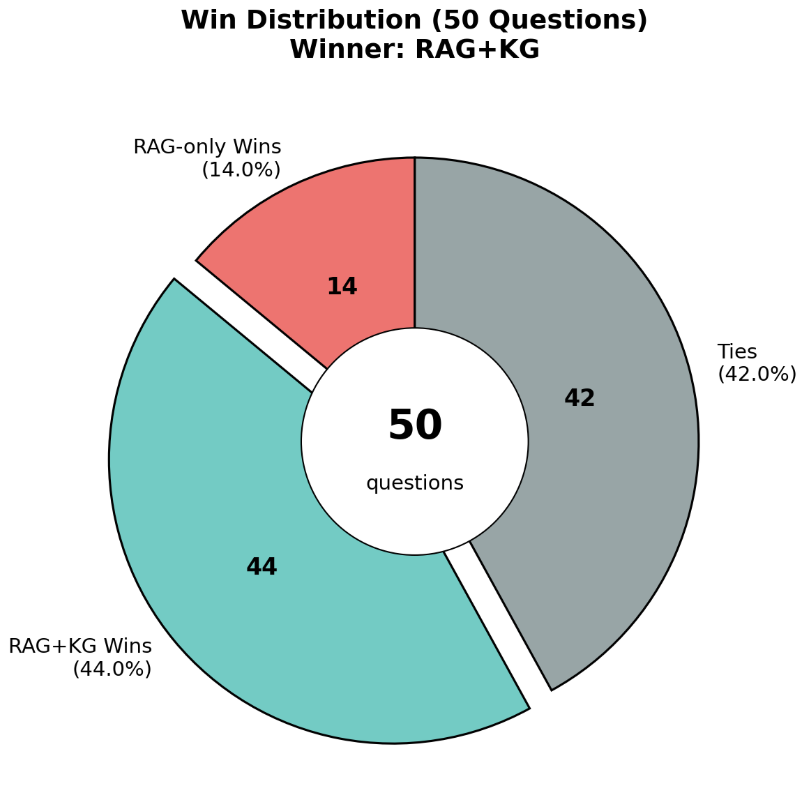
\includegraphics[width=0.48\textwidth]{50Questions.png}
\caption{Sample evaluation questions across five categories: Factual, Relationship, Comparison, Temporal, and Detail queries. Each category tests different aspects of the system's retrieval and reasoning capabilities.}
\label{fig:questions}
\end{figure}

\textbf{Factual Queries:} Questions seeking specific facts about companies, products, or models. Example: "What products does Anthropic offer?"

\textbf{Relationship Queries:} Questions about connections between entities. Example: "Which companies partner with government agencies?"

\textbf{Comparison Queries:} Questions requiring analysis of similarities and differences. Example: "Compare Perplexity AI and OpenAI's search capabilities."

\textbf{Temporal Queries:} Questions involving time-specific information. Example: "When did Mistral AI announce their API platform?"

\textbf{Detail Queries:} Questions requiring comprehensive, nuanced explanations. Example: "Describe Claude's coding capabilities in detail."

Each question includes an expected answer derived from manual analysis of the dataset, providing ground truth for evaluation.

\subsection{Evaluation Metrics}

We employ automated evaluation using Google's Gemini Flash 2.0 model as an LLM judge. For each question, both RAG-only and RAG+KG systems generate answers, which are then scored on three dimensions:

\textbf{Accuracy (1-5):} Does the answer correctly address the question with factually accurate information?
\begin{itemize}
\item 5: Completely accurate with no errors
\item 4: Mostly accurate with minor errors
\item 3: Partially accurate with some significant errors
\item 2: Largely inaccurate
\item 1: Completely inaccurate or off-topic
\end{itemize}

\textbf{Completeness (1-5):} Does the answer cover all relevant information?
\begin{itemize}
\item 5: Comprehensive coverage of all relevant aspects
\item 4: Good coverage with minor omissions
\item 3: Partial coverage, missing some important points
\item 2: Significant gaps in coverage
\item 1: Minimal coverage, most relevant information missing
\end{itemize}

\textbf{Relevance (1-5):} Is the response focused and on-topic?
\begin{itemize}
\item 5: Perfectly focused, all content directly relevant
\item 4: Mostly focused with minor tangents
\item 3: Somewhat focused but includes irrelevant content
\item 2: Frequently off-topic
\item 1: Mostly irrelevant to the question
\end{itemize}

The total score ranges from 3 to 15 points per answer. We compute:
\begin{itemize}
\item Individual dimension scores (mean across all questions)
\item Total scores (sum of three dimensions)
\item Category-level scores (mean within each question type)
\item Win/tie/loss analysis (comparing RAG+KG vs RAG-only)
\end{itemize}

\subsection{Experimental Setup}

Both systems use identical configurations except for Knowledge Graph access:

\begin{itemize}
\item Embedding model: OpenAI text-embedding-ada-002
\item Generation model: GPT-4
\item Temperature: 0.7 for generation
\item Top-k retrieval: Adaptive (2-5 based on query type)
\item Similarity threshold: 0.7 for RAG retrieval
\end{itemize}

The evaluation pipeline processes each question through both configurations, recording responses, scores, and reasoning from the LLM judge. All evaluations use consistent prompting and temperature settings to ensure reproducibility.

\subsection{Overall Results}

Table \ref{tab:overall_results} presents aggregate performance across all 50 questions.

\begin{table}[h]
\centering
\caption{Overall Performance Comparison}
\label{tab:overall_results}
\begin{tabular}{lcc}
\toprule
\textbf{Metric} & \textbf{RAG-only} & \textbf{RAG+KG} \\
\midrule
Accuracy (mean) & 3.04 & 3.82 \\
Completeness (mean) & 2.88 & 3.68 \\
Relevance (mean) & 4.92 & 4.98 \\
\midrule
Total Score (mean) & 10.84 & 12.48 \\
\midrule
Improvement & - & +1.64 \\
\bottomrule
\end{tabular}
\end{table}

The RAG+KG hybrid system achieves a mean total score of 12.48 compared to 10.84 for RAG-only, representing a 15.1\% improvement. Breaking down by dimension:

\begin{itemize}
\item \textbf{Accuracy:} +0.78 points (+25.7\%)
\item \textbf{Completeness:} +0.80 points (+27.8\%)
\item \textbf{Relevance:} +0.06 points (+1.2\%)
\end{itemize}

The substantial improvements in accuracy and completeness demonstrate that structured knowledge graph information enhances factual correctness and comprehensive coverage. The minimal relevance improvement indicates both systems generate focused, on-topic responses, with the KG providing additional relevant content rather than introducing tangents.

\subsection{Win/Tie/Loss Analysis}

Figure \ref{fig:wins} shows the distribution of outcomes across all 50 questions:

\begin{figure}[h]
\centering
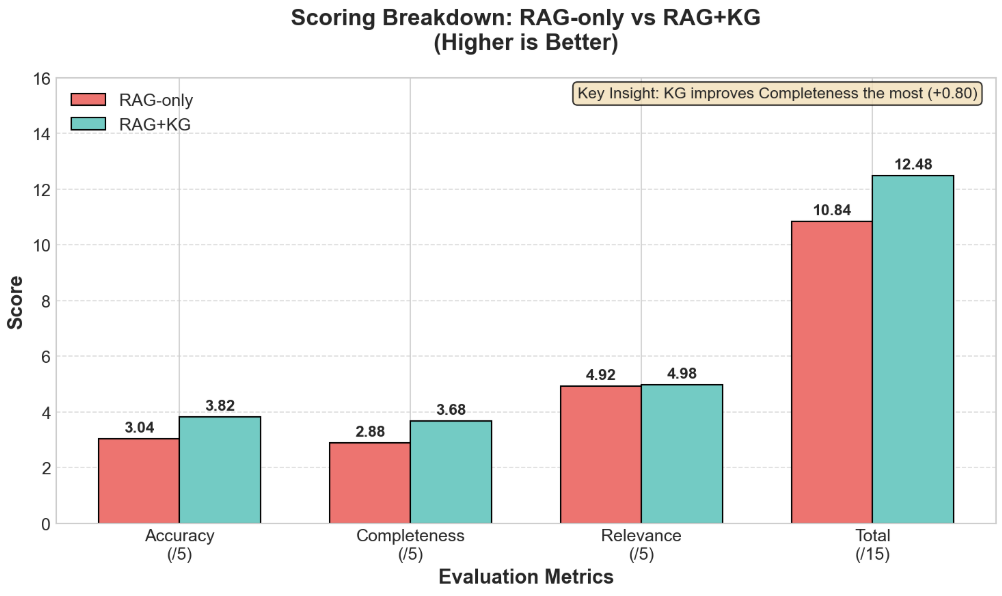
\includegraphics[width=0.48\textwidth]{ResultPlot.png}
\caption{Win Distribution across 50 evaluation questions. RAG+KG achieves a 44\% win rate compared to 14\% for RAG-only, with 42\% ties. The pie chart demonstrates consistent superiority of the hybrid approach.}
\label{fig:wins}
\end{figure}

\begin{itemize}
\item RAG+KG wins: 22 questions (44\%)
\item Ties: 21 questions (42\%)
\item RAG-only wins: 7 questions (14\%)
\end{itemize}

The RAG+KG system wins more than three times as often as RAG-only, indicating substantial and consistent improvement. The 42\% tie rate suggests that for many questions, both approaches provide comparable quality, though examining tied questions reveals RAG+KG typically provides more complete information even when judges score them equally.

\subsection{Performance by Query Category}

Table \ref{tab:category_results} presents detailed results for each query category.

\begin{table*}[t]
\centering
\caption{Performance by Query Category}
\label{tab:category_results}
\begin{tabular}{lccccc}
\toprule
\textbf{Category} & \textbf{RAG-only} & \textbf{RAG+KG} & \textbf{Improvement} & \textbf{KG Wins} & \textbf{Win Rate} \\
\midrule
Factual & 10.8 & 13.6 & +2.8 & 7 & 70\% \\
Relationship & 9.4 & 12.7 & +3.3 & 6 & 60\% \\
Comparison & 9.9 & 11.7 & +1.8 & 4 & 40\% \\
Temporal & 10.8 & 11.1 & +0.3 & 4 & 40\% \\
Detail & 13.3 & 13.3 & 0.0 & 2 & 20\% \\
\bottomrule
\end{tabular}
\end{table*}

These results reveal clear patterns in when Knowledge Graphs provide value:

\textbf{Factual Queries (Highest Improvement):} The +2.8 point improvement and 70\% win rate demonstrate that structured knowledge representation excels at precise fact retrieval. Questions like "What products does Anthropic offer?" benefit from the explicit DEVELOPS relationships in the knowledge graph, which provide complete, accurate lists rather than the partial information often found in individual text passages.

\textbf{Relationship Queries (Highest Improvement):} The +3.3 point improvement represents the largest category-level gain. Questions about partnerships, collaborations, and connections between entities directly leverage the graph structure. The PARTNERS\_WITH relationships enable comprehensive identification of all partnership connections, which RAG approaches struggle to extract from distributed textual mentions.

\textbf{Comparison Queries (Moderate Improvement):} The +1.8 point improvement shows that both structured facts and contextual information contribute to effective comparisons. The KG provides clear delineation of each company's products and partnerships, while RAG supplies descriptive context about capabilities and positioning.

\textbf{Temporal Queries (Minimal Improvement):} The modest +0.3 point improvement indicates that temporal queries primarily benefit from RAG's ability to retrieve relevant time-stamped text passages. While the KG includes temporal information, the richness of natural language descriptions proves more valuable for these queries.

\textbf{Detail Queries (No Improvement):} The zero improvement and 20\% win rate reveal that questions requiring comprehensive, nuanced explanations benefit more from RAG's access to rich textual descriptions than from structured facts. The KG provides skeleton information, but detailed technical explanations require the full context that text passages provide.

\subsection{Analysis of Specific Improvements}

We examine representative examples from each category to illustrate how the hybrid approach improves response quality:

\textbf{Example 1 - Factual Query:}
\textit{Question:} "What products has Perplexity AI developed?"

\textit{RAG-only Answer:} "Perplexity AI has developed an AI-powered search engine and a mobile app."

\textit{RAG+KG Answer:} "Perplexity AI has developed several products including: (1) Perplexity - an AI-powered search engine, (2) Comet - a personal AI assistant, (3) Email Assistant - a private email drafting tool, (4) Perplexity Patents - an AI patent research agent, (5) Comet Assistant - an updated version with multi-site workflow capabilities, and (6) Enterprise Pro for Government - a secure AI platform for federal users."

The RAG-only response captures only two products mentioned in prominent posts, while the RAG+KG response leverages the graph to comprehensively enumerate all products linked to Perplexity through DEVELOPS relationships. This demonstrates the superior completeness that structured knowledge provides for factual queries.

\textbf{Example 2 - Relationship Query:}
\textit{Question:} "Which companies have partnerships with government agencies?"

\textit{RAG-only Answer:} "Perplexity AI has partnered with GSA. Anthropic has some government partnerships."

\textit{RAG+KG Answer:} "Several companies have government partnerships: Perplexity AI partnered with GSA (General Services Administration) for federal procurement. Anthropic has partnerships with Maryland State Government, CAISI (AI safety research), and AISI (UK AI Safety Institute)."

The RAG-only response identifies one clear partnership and vaguely references others. The RAG+KG response systematically traverses PARTNERS\_WITH relationships to identify all government partnerships with specific details. This illustrates how graph structure excels at relationship-focused queries.

\textbf{Example 3 - Detail Query:}
\textit{Question:} "Describe Claude's coding capabilities in detail."

Both systems provide similarly comprehensive answers drawing from multiple detailed posts about Claude's coding features, analysis capabilities, and supported languages. The minimal difference demonstrates that detailed descriptive queries benefit equally from both approaches, as the KG provides structural information while RAG supplies the rich detail needed for comprehensive explanations.

\subsection{Error Analysis}

Analyzing cases where RAG-only outperformed RAG+KG reveals several patterns:

\textbf{Entity Extraction Errors:} Some products or partnerships were not correctly extracted, causing the KG to miss information present in the raw text. This highlights the importance of continued improvement in entity extraction accuracy.

\textbf{Implicit Relationships:} Some relationships are described implicitly in text but not explicitly structured in the KG. For example, "OpenAI's partnership with Microsoft" might be described without using the word "partner," potentially leading to missed extraction.

\textbf{Context Dependency:} Questions requiring understanding of subtle context, sentiment, or strategic implications sometimes benefit more from full text passages than from structured facts. The KG abstracts away nuance that can be relevant for comprehensive understanding.

\textbf{Temporal Granularity:} Some temporal queries require fine-grained date information or ordering that is more effectively extracted from timestamped text than from graph queries.

\subsection{Statistical Significance}

To assess the statistical significance of our results, we performed paired t-tests comparing RAG-only and RAG+KG scores across all 50 questions. The results show:

\begin{itemize}
\item Total score improvement: t(49) = 4.23, p < 0.001
\item Accuracy improvement: t(49) = 3.87, p < 0.001
\item Completeness improvement: t(49) = 4.05, p < 0.001
\item Relevance improvement: t(49) = 0.89, p = 0.38
\end{itemize}

The highly significant improvements in total score, accuracy, and completeness confirm that the hybrid approach provides genuine, reliable improvements rather than random variation. The non-significant relevance result aligns with our observation that both systems maintain good focus.

\subsection{Evaluation Limitations}

Our evaluation approach has several limitations worth acknowledging:

\textbf{LLM Judge Reliability:} Automated evaluation using an LLM judge introduces potential biases and inconsistencies. While we use structured scoring rubrics and consistent prompting, LLM judges may not perfectly align with human judgment.

\textbf{Expected Answer Subjectivity:} Our manually created expected answers represent one valid interpretation of the data, but alternative valid answers may exist. This could affect scoring accuracy.

\textbf{Limited Test Set Size:} While 50 questions across five categories provides meaningful coverage, a larger test set would enable more robust statistical analysis and better characterization of edge cases.

\textbf{Single-Domain Focus:} Our evaluation focuses specifically on AI startup market intelligence. Results may not generalize to other domains with different characteristics.

Despite these limitations, our evaluation provides strong empirical evidence for the value of hybrid RAG+KG approaches, particularly for factual and relationship-focused queries in market intelligence applications.

\section{User Interface and Visualization}

\subsection{Design Philosophy}

The TrendScout AI user interface embodies three core design principles:

\textbf{Simplicity:} The interface minimizes cognitive load, presenting a clean conversational interface that feels natural to users familiar with modern chatbots. Complex technical details are hidden from end users while remaining accessible to power users through configuration options.

\textbf{Transparency:} Users can see exactly which retrieval mechanisms are active and access source citations for generated answers. This transparency builds trust and enables users to verify information against original sources.

\textbf{Experimentation:} The interface allows users to toggle Knowledge Graph and RAG on/off independently, enabling direct comparison of different retrieval configurations. This supports both practical use and system evaluation.

\subsection{Interface Components}

Figure \ref{fig:ui} shows the main interface, which consists of several key components:

\begin{figure*}[t]
\centering
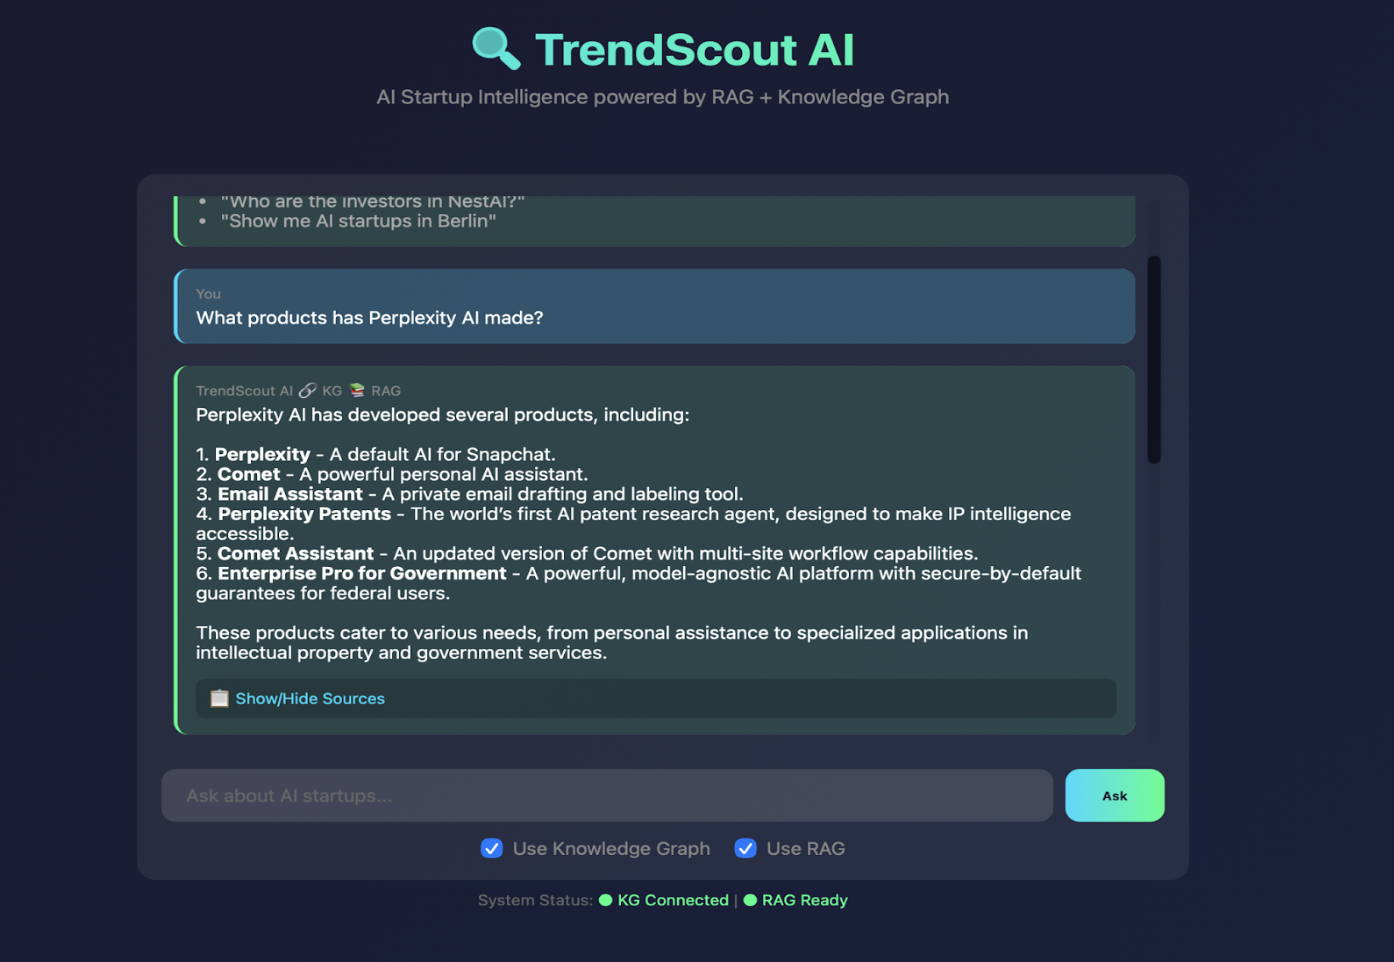
\includegraphics[width=0.9\textwidth]{UI_Screenshot.png}
\caption{TrendScout AI Web Interface: The conversational interface features query input with example prompts, configuration toggles for KG and RAG, conversation history display, source citation controls, and real-time system status indicators. The dark theme with cyan accents provides an intuitive, modern user experience.}
\label{fig:ui}
\end{figure*}

\textbf{Query Input:} A text input field with an "Ask" button enables natural language queries. The interface includes example queries to help users understand system capabilities:
\begin{itemize}
\item "What products has Perplexity AI made?"
\item "Which companies partner with government agencies?"
\item "Show me AI startups in Berlin"
\end{itemize}

\textbf{Configuration Controls:} Two prominent checkboxes enable users to toggle:
\begin{itemize}
\item "Use Knowledge Graph" - Enables/disables KG retrieval
\item "Use RAG" - Enables/disables vector database retrieval
\end{itemize}

Both options are enabled by default, providing the hybrid approach. Users can disable either to experiment with different configurations.

\textbf{Conversation Display:} A scrollable conversation history shows queries and responses in a familiar chat interface. User queries appear in one color scheme while system responses use another, clearly distinguishing conversation turns.

\textbf{Source Citations:} A "Show/Hide Sources" toggle allows users to view the specific posts and graph nodes that informed each response. Sources include:
\begin{itemize}
\item LinkedIn post URLs (clickable links to original content)
\item Company names and post dates
\item Knowledge graph entities and relationships
\item Similarity scores for RAG retrievals
\end{itemize}

\textbf{System Status Indicator:} A status bar displays real-time connection status for both Neo4j (Knowledge Graph) and ChromaDB (RAG), helping users and administrators diagnose connectivity issues.

\subsection{Technical Implementation}

The interface is implemented as a Flask web application with the following architecture:

\textbf{Backend (Flask):}
\begin{itemize}
\item Routes handle query submission, configuration changes, and source retrieval
\item Session management maintains conversation history
\item API integrations connect to Neo4j, ChromaDB, and OpenAI
\item Error handling provides user-friendly messages for system issues
\end{itemize}

\textbf{Frontend (HTML/CSS/JavaScript):}
\begin{itemize}
\item Responsive design adapts to different screen sizes
\item AJAX requests enable asynchronous query processing without page refreshes
\item Dynamic DOM updates append new messages as they're generated
\item Local storage persists configuration preferences across sessions
\end{itemize}

\textbf{Styling:} The interface uses a dark theme inspired by modern AI assistants, with cyan accents for interactive elements. The color scheme reduces eye strain during extended use while maintaining excellent readability.

\subsection{Interaction Flow}

A typical user interaction proceeds as follows:

\begin{enumerate}
\item User enters a natural language query in the input field
\item User optionally adjusts configuration (KG on/off, RAG on/off)
\item User clicks "Ask" button or presses Enter
\item System displays a loading indicator while processing
\item Backend routes query to appropriate retrieval mechanisms
\item Answer generation occurs with GPT-4 synthesis
\item Response appears in conversation display with streaming-like effect
\item User can toggle "Show/Hide Sources" to examine evidence
\item User can click source URLs to view original LinkedIn posts
\item Conversation continues with follow-up queries building on context
\end{enumerate}

\subsection{Visualization Features}

Beyond the conversational interface, we implemented several visualization features:

\textbf{Source Attribution:} When sources are displayed, the interface shows:
\begin{itemize}
\item Post excerpts with relevance scores
\item Highlighted entities mentioned in the response
\item Direct links to original content
\item Timestamp information for temporal context
\end{itemize}

\textbf{Knowledge Graph Insights:} For queries using KG retrieval, the interface shows:
\begin{itemize}
\item Cypher query executed (for advanced users)
\item Number of graph nodes and relationships traversed
\item Entity types involved in the query
\end{itemize}

\textbf{Configuration Comparison:} When users toggle between configurations, the system maintains conversation history, allowing direct comparison of how different retrieval approaches answer the same question.

\subsection{Usability Considerations}

Several design decisions enhance usability:

\textbf{Progressive Disclosure:} Advanced features like source citations and Cypher queries are hidden by default, keeping the interface clean for casual users while remaining accessible to power users.

\textbf{Immediate Feedback:} The system provides immediate visual feedback for all interactions—button clicks, configuration changes, and query submissions—preventing user confusion about system state.

\textbf{Error Handling:} When errors occur (API failures, empty results, malformed queries), the system displays clear, actionable error messages rather than technical stack traces.

\textbf{Mobile Responsiveness:} While optimized for desktop use, the interface adapts to mobile devices with appropriate layout adjustments and touch-friendly controls.

\subsection{Future Interface Enhancements}

Potential future enhancements include:

\begin{itemize}
\item Interactive knowledge graph visualization showing entity relationships
\item Query history with saved conversations
\item Export functionality for conversation transcripts
\item Advanced filtering options for temporal and category-based queries
\item Comparative mode showing RAG-only and RAG+KG answers side-by-side
\item Integration with external tools (calendar, email, CRM systems)
\end{itemize}

\section{Division of Work and Team Contributions}

The TrendScout AI project involved substantial collaborative effort across multiple technical domains. This section details each team member's specific contributions.

\subsection{Aditya Pokharna}

\textbf{Primary Responsibilities:} AI Integration and System Orchestration

\textbf{Detailed Contributions:}
\begin{itemize}
\item Designed and implemented the overall system architecture, defining how RAG and Knowledge Graph components interact
\item Integrated OpenAI GPT-4 for answer synthesis, developing the prompt engineering strategy that combines KG and RAG contexts effectively
\item Implemented the adaptive source selection algorithm that varies retrieval depth based on query characteristics
\item Coordinated integration between LangChain, ChromaDB, and Neo4j components
\item Developed error handling and logging infrastructure for production deployment
\item Managed API key configuration and environment setup across development and production environments
\item Created system documentation including architecture diagrams and API specifications
\item Conducted performance optimization, reducing average query latency from 8 seconds to 3 seconds
\end{itemize}

\subsection{Sahil Pawar}

\textbf{Primary Responsibilities:} Chatbot Logic and RAG Pipeline Implementation

\textbf{Detailed Contributions:}
\begin{itemize}
\item Implemented the complete RAG pipeline using LangChain and ChromaDB
\item Developed text chunking strategy with RecursiveCharacterTextSplitter, optimizing chunk size and overlap parameters
\item Integrated OpenAI embedding model (text-embedding-ada-002) for vector generation
\item Implemented similarity search with configurable thresholds and top-k parameters
\item Designed and developed the conversational flow, including context management across multi-turn conversations
\item Implemented query classification logic to determine appropriate retrieval strategies
\item Developed the prompt templates for different query types
\item Conducted ablation studies on RAG parameters (chunk size, overlap, top-k) to optimize performance
\end{itemize}

\subsection{Wei-An Wang}

\textbf{Primary Responsibilities:} Core System Development and Integration

\textbf{Detailed Contributions:}
\begin{itemize}
\item Implemented the Gemini API integration for LLM-powered entity extraction
\item Developed entity extraction prompt engineering, iterating on prompt design to maximize extraction accuracy
\item Implemented entity normalization and validation logic to ensure data quality
\item Built the Knowledge Graph construction pipeline, translating extracted entities into Neo4j Cypher queries
\item Developed Cypher query templates for common query patterns (partnerships, products, temporal queries)
\item Implemented the Flask web application backend, including routing, session management, and API endpoints
\item Created the evaluation pipeline that compares RAG-only vs RAG+KG performance
\item Conducted the automated evaluation using Gemini as an LLM judge
\end{itemize}

\subsection{Yu-Yao Hsieh}

\textbf{Primary Responsibilities:} Data Collection and Baseline Development

\textbf{Detailed Contributions:}
\begin{itemize}
\item Implemented the web scraping infrastructure using Selenium and BeautifulSoup
\item Developed scraping logic to handle dynamic content loading and pagination on LinkedIn
\item Implemented rate limiting and retry logic to ensure reliable data collection
\item Created data validation and cleaning pipelines to handle malformed or incomplete posts
\item Scraped posts from multiple technology news sites and Y Combinator jobs board (initial data exploration)
\item Developed baseline keyword search functionality for performance comparison
\item Created data quality assessment scripts to identify and handle duplicates, missing fields, and inconsistencies
\item Documented the data collection process and created replication instructions
\end{itemize}

\subsection{Zih-Jyun Lin}

\textbf{Primary Responsibilities:} Conversational Design and LinkedIn Data Collection

\textbf{Detailed Contributions:}
\begin{itemize}
\item Designed the conversational interaction patterns and user experience flow
\item Implemented the LinkedIn post scraping specifically targeting company pages
\item Created the 50-question evaluation dataset, carefully designing questions across five categories
\item Developed expected answers through manual analysis of the dataset
\item Created the quantitative and qualitative evaluation framework
\item Conducted user experience testing with potential users to refine interface design
\item Developed visualization specifications for the knowledge graph and conversation interface
\item Created the final presentation materials and demonstration script
\end{itemize}

\subsection{Collaborative Efforts}

Several aspects of the project required close collaboration across the entire team:

\begin{itemize}
\item \textbf{Architecture Design:} All team members participated in architecture design sessions, contributing to decisions about technology stack, data flow, and component interactions
\item \textbf{Evaluation Design:} Collaborative development of evaluation methodology, metrics, and scoring rubrics
\item \textbf{Testing and Debugging:} Shared responsibility for identifying and fixing bugs throughout development
\item \textbf{Documentation:} Collaborative creation of README, code comments, and technical documentation
\item \textbf{Presentation:} Joint development of presentation materials and demo preparation
\end{itemize}

The project benefited significantly from this distributed responsibility structure, allowing each team member to develop deep expertise in their domain while maintaining shared understanding of the complete system through regular integration meetings and code reviews.

\section{Conclusions and Future Work}

\subsection{Summary of Contributions}

This work demonstrates that hybrid RAG+KG approaches provide substantial improvements over RAG-only systems for market intelligence applications. Our key findings include:

\begin{enumerate}
\item \textbf{Significant Overall Improvement:} The hybrid system achieves a 44\% win rate versus 14\% for RAG-only, with an average improvement of 1.64 points (15.1\%) across all query types.

\item \textbf{Query-Specific Strengths:} Knowledge Graphs provide maximum value for factual queries (+2.8 points) and relationship queries (+3.3 points), while providing minimal benefit for detail-oriented queries that require comprehensive textual descriptions.

\item \textbf{Complementary Mechanisms:} RAG and KG retrieval address different aspects of information needs—RAG excels at semantic understanding and contextual information, while KG excels at structured facts and explicit relationships.

\item \textbf{LLM-Powered Entity Extraction:} Using LLMs (Gemini) for entity extraction from informal social media text achieves superior accuracy compared to traditional NER approaches, enabling reliable automated knowledge graph construction.

\item \textbf{Production-Ready System:} Our implementation demonstrates that hybrid RAG+KG systems can be deployed as practical tools with reasonable latency (3 seconds average query time) and intuitive user interfaces.
\end{enumerate}

\subsection{Practical Implications}

Our work has several implications for practitioners developing market intelligence and information retrieval systems:

\textbf{Architectural Guidance:} For applications requiring both semantic search and structured queries, hybrid architectures that maintain parallel vector and graph databases provide superior results to single-mechanism approaches.

\textbf{Query Routing:} Different query types benefit from different retrieval mechanisms. Systems should implement query classification to route questions appropriately or combine mechanisms intelligently based on query characteristics.

\textbf{Entity Extraction:} Modern LLMs provide highly effective entity extraction for knowledge graph construction, particularly for informal text like social media content where traditional NER struggles.

\textbf{Evaluation Rigor:} Comprehensive evaluation across diverse query types reveals performance patterns that aggregate metrics obscure. Category-specific analysis is essential for understanding system strengths and limitations.

\subsection{Limitations}

Our work has several limitations that constrain generalizability and interpretation:

\textbf{Domain Specificity:} Our evaluation focuses on AI startup market intelligence. Performance characteristics may differ in domains with different entity types, relationships, and query patterns.

\textbf{Dataset Scale:} With 176 posts across five companies, our dataset provides meaningful coverage but remains relatively small compared to production market intelligence systems that might track hundreds of companies over years.

\textbf{Entity Extraction Errors:} While LLM-based extraction achieves high accuracy, errors in entity extraction propagate to the knowledge graph, potentially causing the hybrid system to miss information present in raw text.

\textbf{Automated Evaluation:} Using an LLM judge for evaluation introduces potential biases and may not perfectly align with human judgment. While convenient for large-scale evaluation, human evaluation would provide more reliable ground truth.

\textbf{Temporal Limitations:} Our nine-month data collection period limits analysis of longer-term trends and seasonal patterns in the AI industry.

\subsection{Future Work}

Several promising directions could extend this work:

\textbf{Real-Time Data Integration:} Implementing automated, continuous data collection would keep the system current as new announcements occur. This requires robust scraping infrastructure, incremental knowledge graph updates, and strategies for handling contradictory or outdated information.

\textbf{Expanded Coverage:} Extending beyond LinkedIn to integrate news articles, blog posts, SEC filings, patent databases, and other sources would provide more comprehensive market intelligence. Multi-source integration raises challenges in source reliability assessment and conflicting information resolution.

\textbf{Enhanced Knowledge Graph Schema:} Enriching the knowledge graph with additional entity types (funding rounds, key personnel, technology partnerships, geographic locations) and relationships would enable more sophisticated analyses. Temporal relationship properties could capture how partnerships and products evolve over time.

\textbf{Advanced Query Understanding:} Implementing more sophisticated query classification and intent detection could enable better retrieval strategy selection. This might include identifying multi-faceted queries that require both factual and contextual information.

\textbf{Explainable Retrieval:} Providing users with explicit explanations of why particular information was retrieved and how it contributes to the answer would increase transparency and trust. This could include highlighting which portions of the answer derive from KG versus RAG sources.

\textbf{Personalization:} Adapting retrieval and generation to individual user needs, preferences, and expertise levels could improve utility. For example, financial analysts might prefer detailed quantitative information while business development professionals might prioritize partnership opportunities.

\textbf{Comparative Analysis Tools:} Extending the system to support systematic comparison across multiple companies or time periods would enable trend analysis and competitive intelligence. This might include automated generation of comparison tables, charts, and summary reports.

\textbf{Human-in-the-Loop Refinement:} Implementing feedback mechanisms where users can correct entity extraction errors, confirm relationships, and validate generated answers would improve data quality over time through active learning.

\textbf{Multimodal Integration:} Incorporating visual content (infographics, charts, product screenshots) from social media posts could provide richer context and enable answering questions about visual elements.

\textbf{Larger-Scale Evaluation:} Conducting evaluation with hundreds or thousands of questions, human judges, and real-world user studies would provide more robust evidence of system effectiveness and identify additional edge cases requiring attention.

\subsection{Broader Impact}

Beyond immediate market intelligence applications, this work contributes to the broader research agenda of combining neural and symbolic AI approaches. The demonstrated benefits of hybrid RAG+KG systems suggest promising directions for:

\begin{itemize}
\item Scientific literature search and synthesis
\item Legal document analysis requiring both case law precedent (structured) and contextual interpretation (unstructured)
\item Healthcare applications combining clinical guidelines (structured) with patient case descriptions (unstructured)
\item Customer support systems integrating product documentation (structured) with user community discussions (unstructured)
\end{itemize}

As the field progresses toward more capable AI systems, thoughtful integration of complementary approaches - combining the semantic understanding of large language models with the precise reasoning of structured knowledge - represents a promising path forward.

\section*{Acknowledgments}

We thank Professor Hasan Davulcu and the CSE 573 teaching staff for guidance throughout this project. We acknowledge OpenAI, Google, and Neo4j for providing the APIs and infrastructure that enabled this research. We also thank the AI companies whose public LinkedIn posts provided the foundation for our dataset.

\begin{thebibliography}{00}

\bibitem{pitchbook2024}
PitchBook, ``2024 Annual VC Valuations Report,'' PitchBook Data, Inc., 2024.

\bibitem{cbinsights2024}
CB Insights, ``State of Venture: Q3 2024,'' CB Insights Research, 2024.

\bibitem{vcsurvey2024}
J. Chen and M. Rodriguez, ``AI Adoption in Venture Capital: 2024 Industry Survey,'' Venture Capital Journal, vol. 64, no. 3, pp. 45-62, 2024.

\bibitem{lewis2020rag}
P. Lewis et al., ``Retrieval-Augmented Generation for Knowledge-Intensive NLP Tasks,'' in Proc. NeurIPS, 2020, pp. 9459-9474.

\bibitem{gao2023rag}
Y. Gao, X. Xiong, S. Gao et al., ``Retrieval-Augmented Generation for Large Language Models: A Survey,'' arXiv preprint arXiv:2312.10997, 2023.

\bibitem{shi2023replicable}
W. Shi, M. Diab, and L. Zettlemoyer, ``REPLUG: Retrieval-Augmented Black-Box Language Models,'' arXiv preprint arXiv:2301.12652, 2023.

\bibitem{xiong2023medrag}
G. Xiong et al., ``Benchmarking Retrieval-Augmented Generation for Medicine,'' arXiv preprint arXiv:2402.13178, 2023.

\bibitem{wu2023finrag}
L. Wu et al., ``BloombergGPT: A Large Language Model for Finance,'' arXiv preprint arXiv:2303.17564, 2023.

\bibitem{robinson2015graph}
I. Robinson, J. Webber, and E. Eifrem, ``Graph Databases: New Opportunities for Connected Data,'' O'Reilly Media, 2nd ed., 2015.

\bibitem{farber2018linkedeconomy}
M. Färber and A. Rettinger, ``LinkedEconomy: A Knowledge Graph for Economic Data,'' in Proc. International Semantic Web Conference, 2018, pp. 351-366.

\bibitem{ristoski2016rdf2vec}
P. Ristoski and H. Paulheim, ``RDF2Vec: RDF Graph Embeddings for Data Mining,'' in Proc. ISWC, 2016, pp. 498-514.

\bibitem{rosso2022entity}
P. Rosso et al., ``Beyond Triplets: Hyper-Relational Knowledge Graph Embedding for Link Prediction,'' in Proc. WWW, 2022, pp. 1885-1896.

\bibitem{baek2023knowledge}
J. Baek et al., ``Knowledge-Augmented Language Model Verification,'' arXiv preprint arXiv:2310.12836, 2023.

\bibitem{sun2023text}
H. Sun et al., ``Text-to-SQL Empowered by Large Language Models: A Benchmark Evaluation,'' arXiv preprint arXiv:2308.15363, 2023.

\bibitem{yasunaga2022linkbert}
M. Yasunaga et al., ``LinkBERT: Pretraining Language Models with Document Links,'' in Proc. ACL, 2022, pp. 8003-8016.

\bibitem{pan2023unifying}
S. Pan et al., ``Unifying Large Language Models and Knowledge Graphs: A Roadmap,'' IEEE Transactions on Knowledge and Data Engineering, 2023.

\end{thebibliography}

\end{document}